% id: 14-12
% book: 베이직쎈 확률과 통계 · 01 여러 가지 순열
% section: 개념 03 최단 거리로 가는 경우의 수
% passage: 다음 그림과 같은 도로망이 있다. $\pt{A}$에서 $\pt{B}$까지 최단 거리로 가는 경우의 수를 구하시오.
% figure: tikz:fig-14-12
% answer: 
% answer_source: 
% variant_level: 0 (원본 전사)
% 이 파일은 build.mjs 가 items.json 에서 만든다. 고칠 때는 items.json 을 고친다.
\smash{\raisebox{1.5mm}{\dmkichul{베이직쎈 확률과 통계 14쪽 12번}}}
\noindent\begin{minipage}[t]{0.58\linewidth}\vspace{0pt}\raggedright \end{minipage}\hfill\begin{minipage}[t]{0.4\linewidth}\vspace{0pt}\centering \resizebox{\ifdim\width>\linewidth\linewidth\else\width\fi}{!}{% 14-12(본책 14쪽) — 가로 2칸·세로 1칸 도로망(A 왼쪽 아래 · B 오른쪽 위). 스캔 그림을 TikZ 로 다시 그림(스캔 화질).
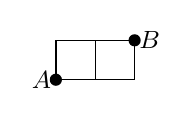
\begin{tikzpicture}[line width=0.5pt]
  \foreach \x in {0, 0.5, 1} { \draw (\x,0) -- (\x,0.5); }
  \foreach \y in {0, 0.5} { \draw (0,\y) -- (1,\y); }
  \fill (0,0) circle (2.2pt);
  \node[left, font=\small, inner sep=1.5pt] at (0,0) {$\pt{A}$};
  \fill (1,0.5) circle (2.2pt);
  \node[right, font=\small, inner sep=1.5pt] at (1,0.5) {$\pt{B}$};
\end{tikzpicture}
}\end{minipage}\par
\dmhint{$\pt{A}$에서 $\pt{B}$까지 최단 거리로 가려면 오른쪽으로 $\blank$칸, 위쪽으로 $\blank$칸 이동해야 한다.\\ 오른쪽으로 1칸 가는 것을 $a$, 위쪽으로 1칸 가는 것을 $b$라 하면 최단 거리로 가는 경우의 수는 $a$, $a$, $\blank$를 일렬로 나열하는 경우의 수와 같다.\\ 따라서 구하는 경우의 수는 $\dfrac{3!}{\blank!}=\blank$}
